\setchapterpreamble[u]{\margintoc}
\chapter{Findings: Analytics in Use}

This chapter presents the research findings based on two of the six perspectives: \uuse and \iuse, \emph{i.e.} how app developers currently use mobile analytics and ways the use could be improved. Figure \ref{fig:dev-practices-with-mobile-analytics} provides the visual context of the development practices and artefacts~\footnote{This figure will be revised pre-submission and keyed into the contents of this chapter. Versions of this figure may feature throughout the thesis with the pertinent elements highlighted and less relevant elements diminished or hidden from view.}.

\begin{figure}
    \centering
    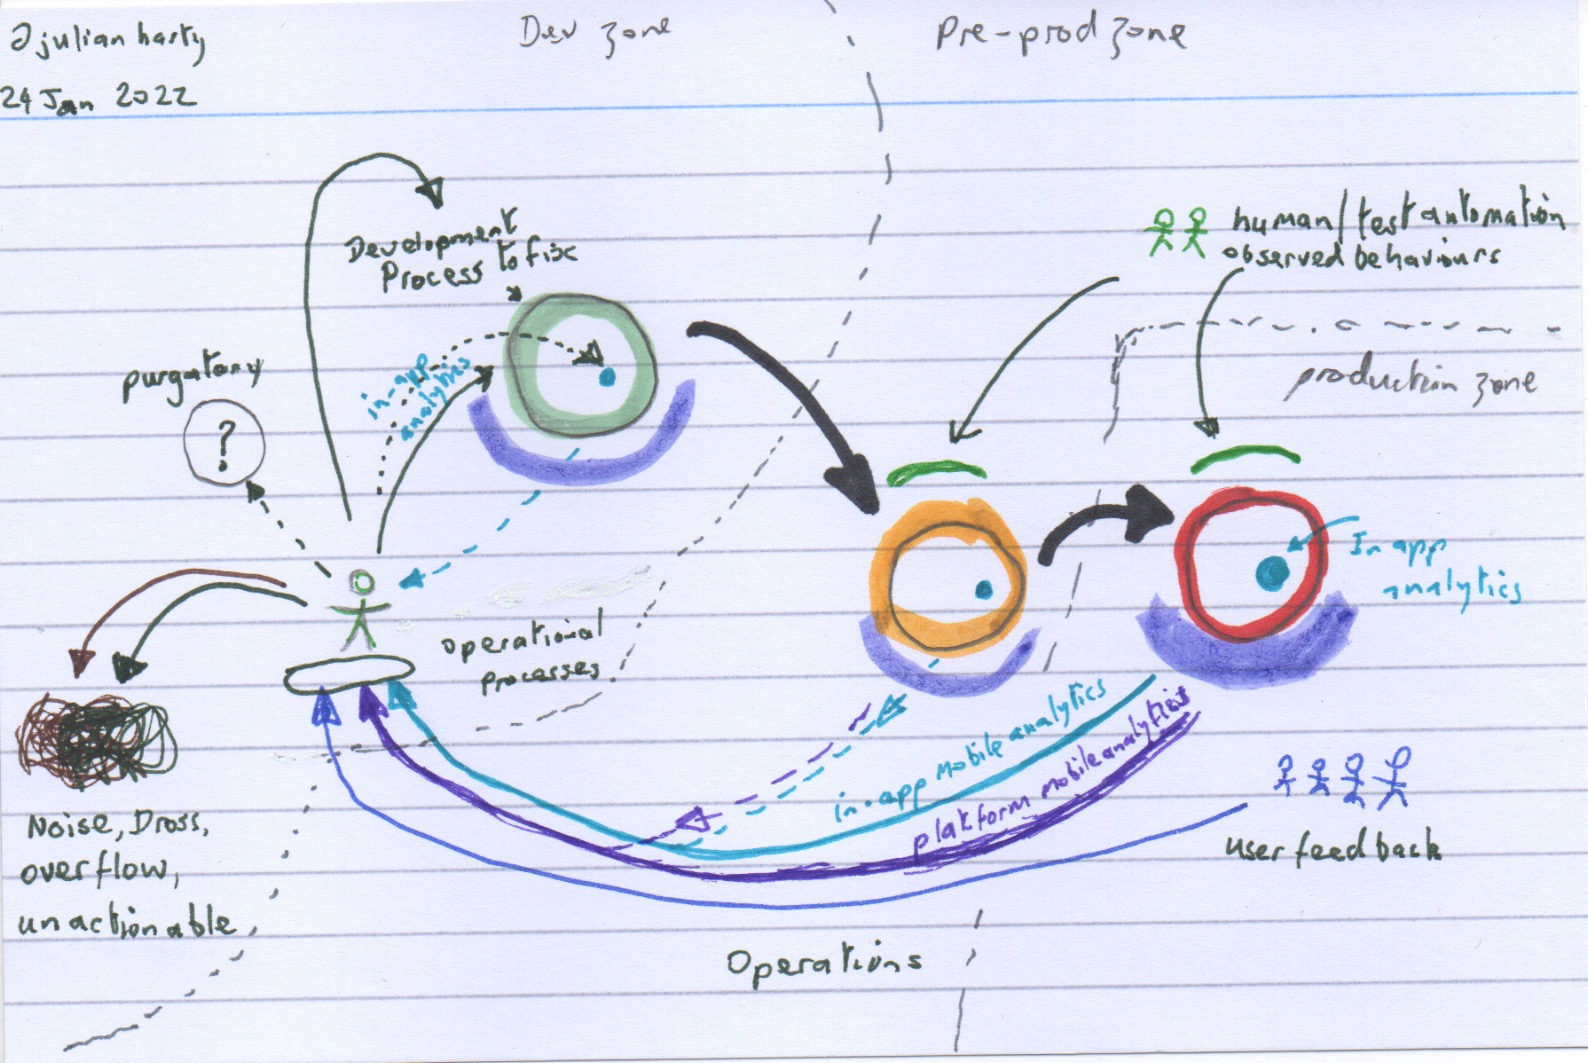
\includegraphics[width=\linewidth]{images/rough-sketches/dev-practices-with-mobile-analytics-24-jan-2022.jpeg}
    \caption{Dev Practices with Mobile Analytics}
    \label{fig:dev-practices-with-mobile-analytics}
\end{figure}

Figure \ref{fig:dev-practices-with-mobile-analytics} has:
\begin{itemize}
\item Three zones: dev, pre-production, and production. Developers are in the dev zone where they work on tasks and create release candidates of their mobile app(s). 
\item The release candidates are illustrated by a coloured circle. 
    \begin{itemize}
    \item Green are releases in the safe zone, within the development zone. These are easy to work with and easy to cease.
    \item Amber releases are in the pre-release zone, they may be used by people external to the development team \textit{e.g.} colleagues, senior managers, closed, and/or open groups of users. The releases require some additional management to control the release rollout, some additional support, and they're harder to cease \textit{i.e.} to stop them from being used. App stores and/or third-party services may help make the releases available to these users.
    \item Red releases are in the production zone, they can be used by anyone who downloads them from the app store. Once releases reach production they can be extremely hard to cease entirely. In practice users are found who use years-old releases even after any mechanisms have been enabled to prevent those releases from functioning. 
    \end{itemize}
\item Within each release candidate developers can choose to incorporate one or more in-app mobile analytics libraries as part of a mobile analytics SDK. In the diagram the in-app mobile analytics libraries are represented by a small aquamarine spot. As the release candidate moves from development to pre-production usage is likely to increase somewhat, and as the release candidate is promoted into production the usage increases significantly, often by orders of magnitude for popular apps. The purple arcs under the circles represent the feedback being generated by the usage of that release of the app.
\item TBC...
\end{itemize}


\begin{figure*}
    \centering
    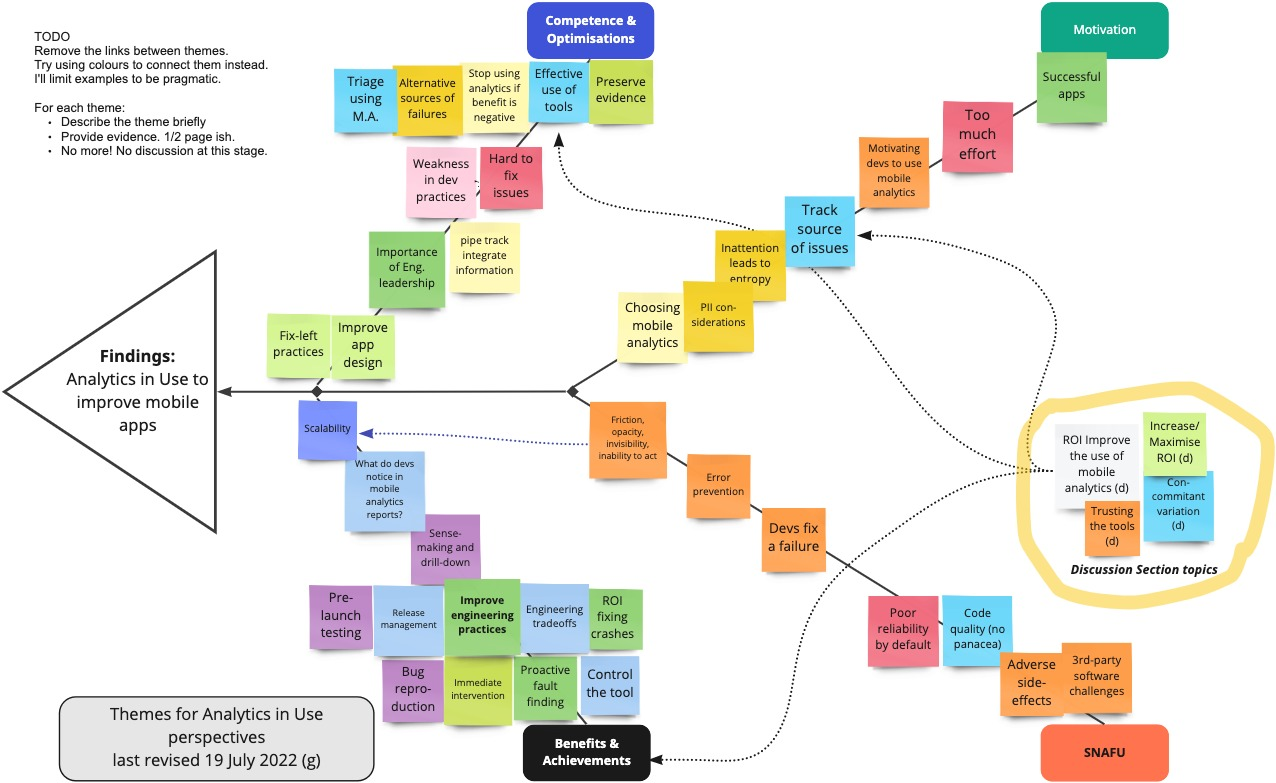
\includegraphics[width=\linewidth]{images/rough-sketches/analytics-in-use-fishbone-diagram-19-jul-2022g.jpeg}
    \caption{Analytics-in-Use fishbone diagram\\Source:~\href{https://miro.com/app/board/uXjVOlelPDU=/?share_link_id=219460632025}{MIRO board diagram}.}
    \label{fig:analytics-in-use-fishbone-diagram}
\end{figure*}

\section{Motivating factors}~\label{aiu-motivating-factors-section}